\documentclass[pdf, hyperref={unicode}, aspectratio=169]{beamer}

\usepackage{styles}
\usepackage{mathtools}

\usepackage{wrapfig}
\usepackage{lipsum}


\DeclarePairedDelimiter\ceil{\lceil}{\rceil}
\DeclarePairedDelimiter\floor{\lfloor}{\rfloor}

\title{Вычисление интерполяционного многочлена Лагранжа}

\subtitle{Лабораторная работа по курсу "Архитектура суперкомпьютеров и вычислительных кластеров"}

\pdfstringdefDisableCommands{
  \def\\{}
  \def\,{}
  \def\textbf#1{<#1>}
}

\author[Спиридонов Кирилл Анатольевич]
{
  \textbf{Студент группы М8О-107М-23:} Спиридонов Кирилл Анатольевич\\
  \ \textbf{Преподаватель курса: } С.\,В.\,Стрижак
}

\institute[Московский авиационный институт]
{
  Московский авиационный институт (национальный исследовательский университет)\\
  Институт № 8 «Компьютерные науки и прикладная математика»\\
  Кафедра № 806 «Вычислительная математика и программирование» 
}

\date{Москва --- \the\year}

\logo{
\includegraphics[height=1cm]{images/mai.pdf}}

\usepackage{lipsum}
\usepackage{animate}


\begin{document}

{
% убирает номер слайда с титульного слайда
\setbeamertemplate{page number in head/foot}{}
\frame{\titlepage}
}

\begin{frame}
\frametitle{Постановка задачи}


Пусть заданы значения функции $y = f (x)$ на некотором множестве точек из области определения

$$
    \Delta = \{(x_i, y_i), x_i \in D, y_i = f(x_i), 0 \le i \le n\}
$$

Точки $x_i$, $0 \le i \le n $ называются узлами интерполяции. Величина $\delta x_i = x_i - x_{i-1}$ называется шагом интерполяционной сетки, который может быть как постоянным, так и переменным. Кроме того, могут быть заданы дополнительные значения, например, значения производных. Тогда задача интерполяции состоит в поиске такой функции $f_\Delta(x)$ из заданного класса функций $F$, что $y_i = f_\Delta(x_i), 0 \le i \le n$.

\end{frame}


\begin{frame}
\frametitle{Полином Лагранжа}

Рассмотрим метод интерполяции с использованием многочленов Лагранжа. Представим интерполяционную функцию в виде полинома
$$
    P_n = \sum_{i=0}^{n} y_iL_{n, i}(x),
$$

где $L_{n, i}(x)$ - полиномы степени n вида:

$$
    L_{n, i}(x) = \prod_{j = 0, j \neq i}^{n} \frac{x - x_j}{x_i - x_j}
$$

Полином $L_{n, i}(x)$ принимает значение 1 в точке $x_i$ и $0$ в остальных узлах интерполяции. Следовательно, в точке $x_i$ исходный полином принимает значение $y_i$.

\end{frame}



\begin{frame}
\frametitle{Алгоритм распараллеливания}

\begin{itemize}

\item N - количество точек, в которых необходимо посчитать значение функции
\item n - количество улов интерполяции
\item p - количество процессов

\end{itemize}

В каждый процесс передаём узлы интерполяции и $\ceil*{\frac{N}{p}}$ точек для расчёта функции $P(x)$. При таком подходе только $N \mod p$ процессов будут простаивать на последней итерации.

\textbf{Сложность алгоритма:} $O( Nn^2 / p)$


\end{frame}


\begin{frame}
\frametitle{Результаты работы}


\begin{figure}%
    \centering
    \subfloat{{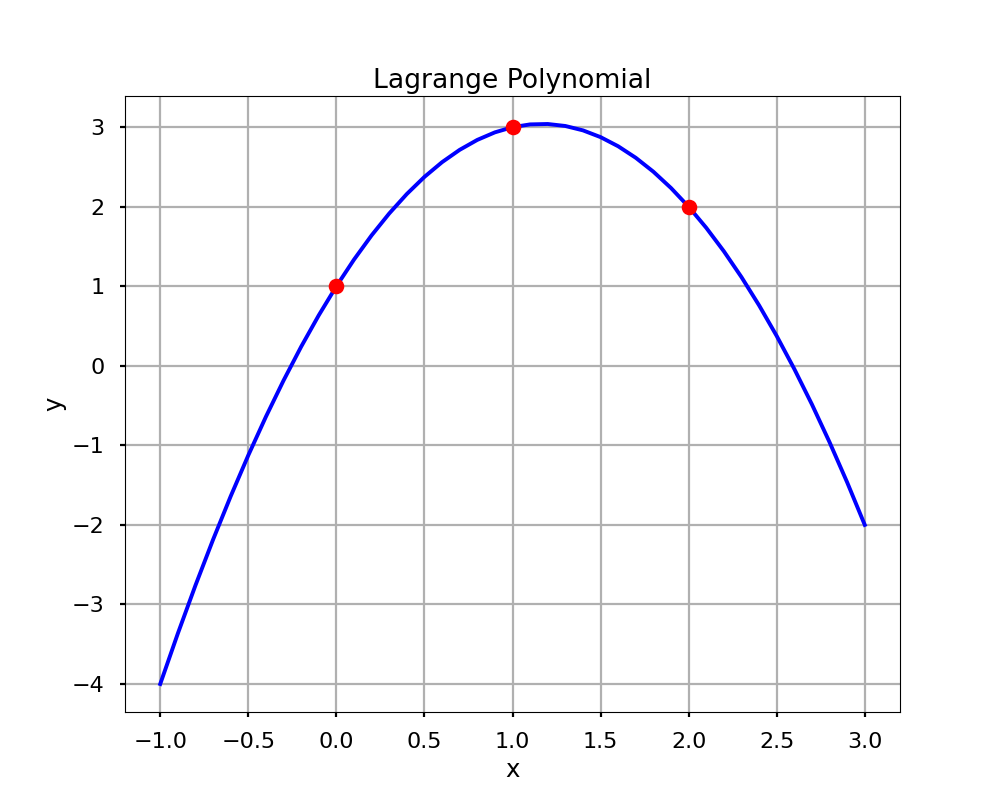
\includegraphics[scale=0.22]{images/example_01.png} }}%
    \qquad
    \subfloat{{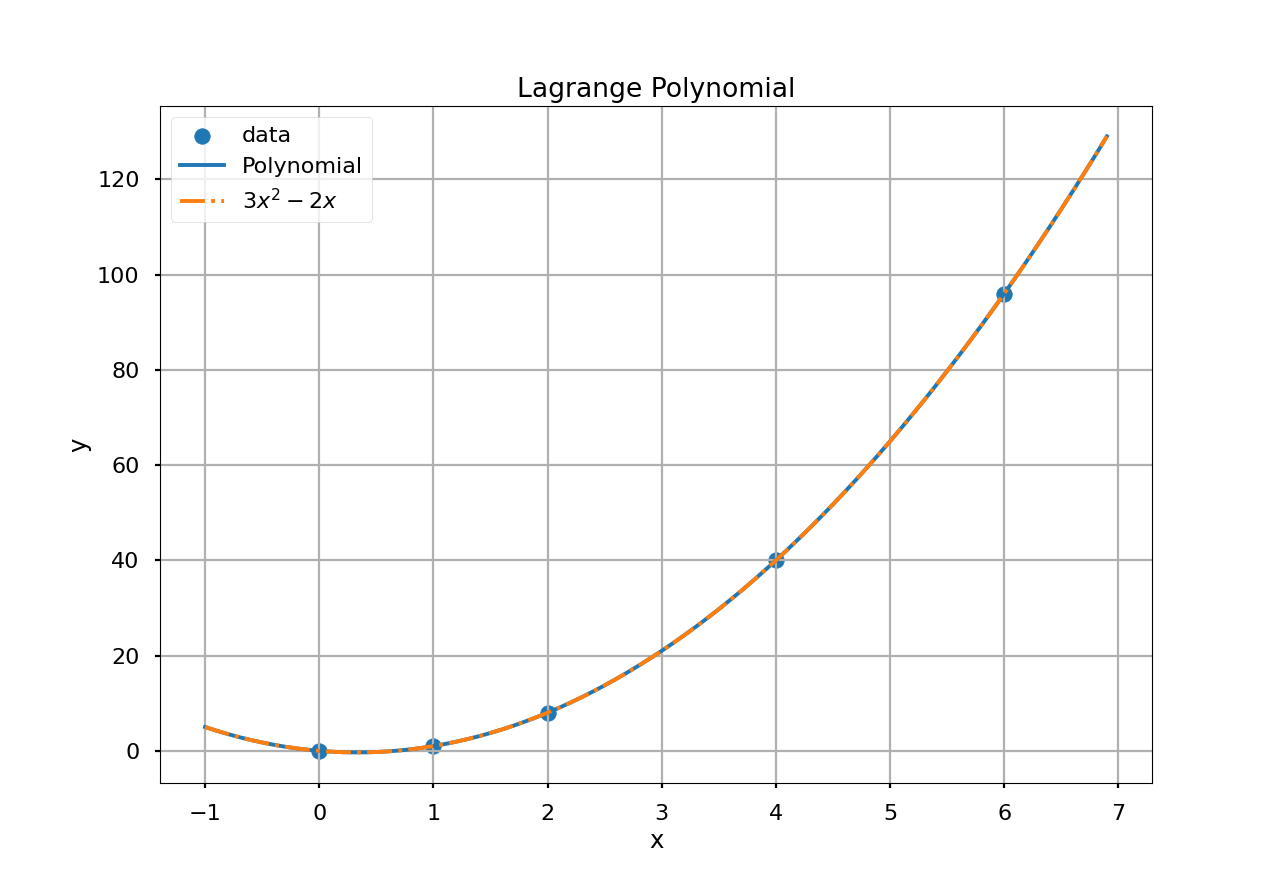
\includegraphics[scale=0.22]{images/example_02.png} }}%
    \label{fig:example}%
\end{figure}

\end{frame}


\begin{frame}
\frametitle{Стек технологий}


% \begin{wrapfigure}{r}{7cm}
Измерения производились при N = 1000, n = 1000.
Время выполнения непараллельной программы $\approx 45$ сек.

\centering
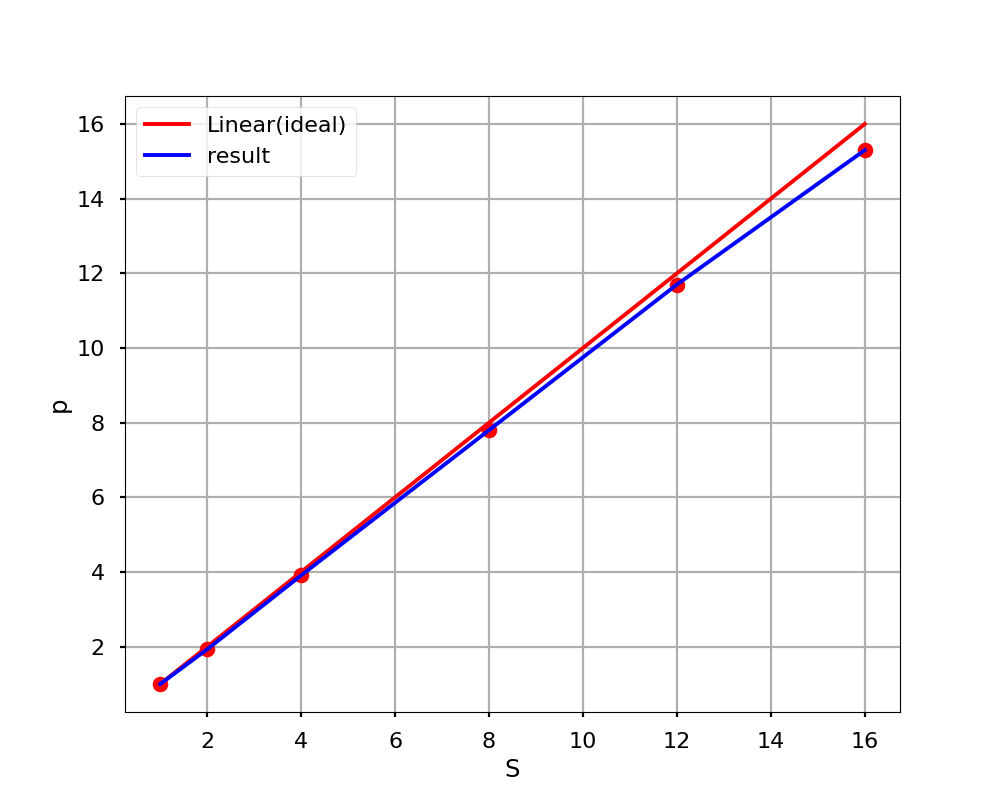
\includegraphics[scale=0.3]{images/speedup.png}
% \end{wrapfigure}

\end{frame}

\end{document}
